\section{Action-Contract Development Diagnostics}
\label{app:action-diagnostics}

The v3 protocol validated the three actions central to the claimed
rebalancing mechanism, but it did not require scale-up and scale-down.  We
therefore declared a stricter v4 gate before running a new study. Each of
$a^{\mathrm{reb}N}$, $a^{\mathrm{reb}G}$, $a^{\mathrm{scale}+}$,
$a^{\mathrm{scale}-}$, and $a^{\mathrm{mig}}$ had to be selected in at least
$80\%$ of admissible episodes in its own fixed validation scenario. Every
candidate also had to pass four probe and telemetry fault guards.  Five seeds were
trained for $20{,}000$ transitions with uniform replay and again with
action-stratified replay, giving $100{,}000$ exact training transitions in each
development run.

\begin{figure}[t]
  \centering
  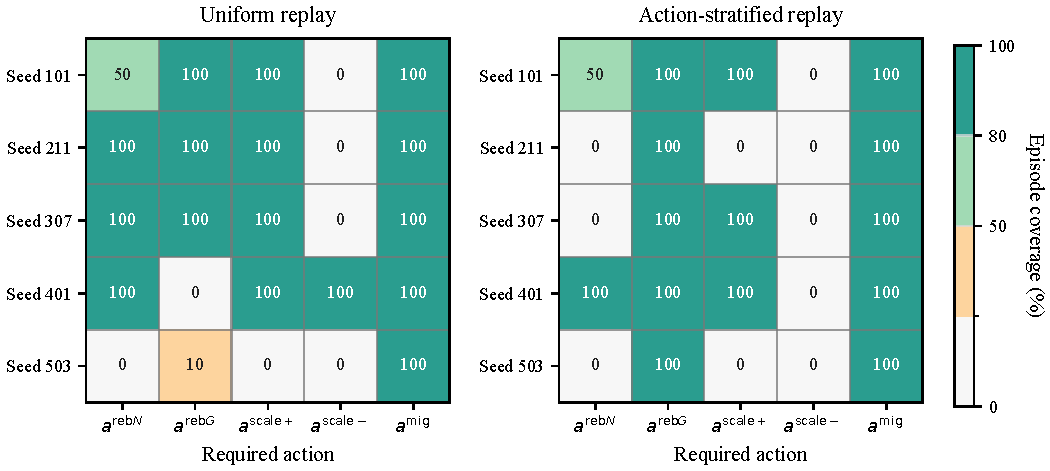
\includegraphics[width=\textwidth]{figures/v4-action-coverage.pdf}
  \caption{Fixed-validation episode coverage for required actions in the two
  v4 development runs.  A cell gives the percentage of admissible episodes in
  which the frozen candidate selected the indicated action; the predeclared
  pass threshold was $80\%$ for every column in one row.}
  \Description{Two five-by-five square heatmaps compare uniform and
  action-stratified replay.  Rows are candidate seeds and columns are the five
  required intervention actions.  A vertical color bar ranges from zero to one
  hundred percent.  No row reaches at least eighty percent in all five columns,
  primarily because scale-down remains zero.}
  \label{fig:v4-action-coverage}
\end{figure}

All ten candidates passed the scripted scenario-feasibility checks and every
fault-safety contract. No row in
Figure~\ref{fig:v4-action-coverage} passes all five policy-coverage conditions.
Uniform-replay seed 401 exercises scale-down but misses backlog rebalancing;
the other uniform candidates miss scale-down.  Every action-stratified
candidate misses scale-down, and several also miss subscription rebalancing or
scale-up. Action-stratified replay left gaps in frozen-policy action coverage.
Under the declared stopping rule, both v4 studies ended at the development
gate and retained their checkpoints for diagnosis. Their results concern
action coverage rather than new holdout performance estimates.

V5 then changed only the scale-down admissibility rule and used fresh candidate
and validation seeds. The historical target-metric checks passed, including a
$49.6\%$ connection-cost reduction for scale-down. All five frozen candidates passed every fault guard and
selected $a^{\mathrm{reb}G}$, $a^{\mathrm{scale}+}$, and
$a^{\mathrm{mig}}$ in all ten intended validation episodes.  However, each
selected $a^{\mathrm{reb}N}$ and $a^{\mathrm{scale}-}$ in zero of ten intended
episodes.  For the diagnostic candidate with the best reward, we evaluated each missed
action for one step from the same state. Both improved reward, but its Q-values ranked \emph{stay}
higher. A later audit showed that the old $a^{\mathrm{scale}+}$ action reduced
its declared maximum-subscription metric by $21.78\%$ but lowered mean scalar
reward by 0.04946 relative to static placement. The v5 diagnostics therefore
distinguish missed one-step reward gains from a scale-up implementation that
conflicted with its reward objective. The coverage gate was not met, and the
study ended without a holdout evaluation.

V6 changed only the scale-up contract. The revised $a^{\mathrm{scale}+}$ opens
one connection and performs bounded, receipt-gated $a^{\mathrm{reb}N}$ moves
until the subscription target is restored or no eligible move remains. In the
locked ten-seed preflight, the option improved mean interval reward by 0.04350
with a paired bootstrap 95\% interval of [0.03559, 0.05114]. It reduced the
mean maximum subscriptions per connection by 38.824, with interval [-38.824,
-38.824]. Every episode restored the target using exactly 50 moves, without an
executor no-op or scale-down reversal. This scripted preflight verifies the
revised action contract in the simulator; learned selection is evaluated in
the study below.

The locked v6 study then tested each combination of Target-Max or Double-DQL
bootstrapping with squared or Huber temporal-difference loss. Each arm trained five fresh
candidates for $20{,}000$ transitions and evaluated them on ten fresh
development-validation seeds. Table~\ref{tab:v6-factorial-coverage} reports
the number of candidates passing each action gate. Every candidate passed all
four safety scenarios, but no candidate passed all five action gates. The
predeclared requirement of at least four fully eligible candidates was
therefore unmet in every arm. No policy was selected and no holdout was defined
or executed. Squared and Huber loss magnitudes are not ranked against each
other because the two losses have different numerical scales.

\begin{table}[t]
  \caption{V6 development-gate results. Each action and safety entry is the
  number of passing candidates out of five. TM denotes Target-Max bootstrap;
  DDQL denotes Double-DQL. An arm required at least four candidates that each
  passed all action and safety gates.}
  \Description{Four rows report action coverage and safety counts for the v6
  Target-Max and Double-DQL arms with squared and Huber losses. Every arm has
  zero fully eligible candidates. All safety counts are five, while scale-up is
  zero except for one passing candidate in the Target-Max Huber arm.}
  \label{tab:v6-factorial-coverage}
  \centering
  \small
  \setlength{\tabcolsep}{3pt}
  \begin{tabular}{llccccccc}
    \toprule
    Arm & Learner/loss & Eligible & $a^{\mathrm{reb}N}$ & $a^{\mathrm{reb}G}$ & $a^{\mathrm{scale}+}$ & $a^{\mathrm{scale}-}$ & $a^{\mathrm{mig}}$ & Safety \\
    \midrule
    A & TM/squared & 0 & 0 & 1 & 0 & 5 & 5 & 5 \\
    B & DDQL/squared & 0 & 2 & 2 & 0 & 5 & 5 & 5 \\
    C & TM/Huber & 0 & 3 & 5 & 1 & 5 & 5 & 5 \\
    D & DDQL/Huber & 0 & 4 & 5 & 0 & 5 & 5 & 5 \\
    \bottomrule
  \end{tabular}
\end{table}

\FloatBarrier
The cap-restoring executor improves the fixed reward, while learned selection
varies across candidates. The diagnostics distinguish the corrected action
contract from policy coverage. They leave the individual effects of value
estimation, visited states, replay sampling, and credit across several moves
unresolved.
